% fixture: tikz/figure-pdftex
% oracle: pdflatex
% tier: T3
% engine: document
% specials: compare
% covers: tikzpictures in figures (two side by side with \hfill) with \centering and a caption; coordinates by name, polar and relative coordinates, to, |- and -|; a clip
% issue: #309
\documentclass{article}
\usepackage{tikz}
\usetikzlibrary{positioning,arrows.meta}
\begin{document}
Some text before the figure, long enough to make a line or so of a paragraph here.
\begin{figure}[h]
  \centering
  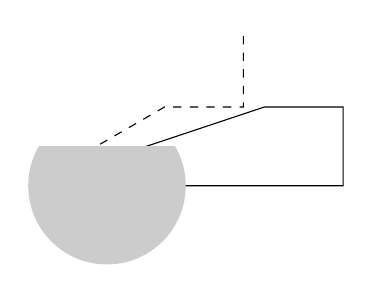
\begin{tikzpicture}
    \coordinate (a) at (0,0);
    \coordinate (b) at (3,1);
    \draw (a) -- (b) -| (4,0) |- (a);
    \draw[dashed] (a) to (30:2cm) to ++(1,0) -- +(0,1);
    \clip (0,-1) rectangle (2,0.5);
    \fill[gray!40] (1,0) circle (1);
  \end{tikzpicture}
  \caption{A figure drawn with TikZ.}
\end{figure}
The text goes on after the figure.
\begin{figure}[h]
  \centering
  
\begin{tikzpicture}\draw (0,0) rectangle (2,1);\end{tikzpicture}\hfill
  
\begin{tikzpicture}\fill[blue!20] (0,0) circle (0.5);\end{tikzpicture}
  \caption{Two pictures side by side.}
\end{figure}
And a last paragraph.
\end{document}
